\chapter{The Basic Laws To Maxwell's Equation (1)}\label{lec:lec18}


\begin{mdframed}[backgroundcolor=lightblue, linewidth=1pt, hidealllines=true]
\section{Objectives}
By the end of this chapter, you should be able to:
\begin{enumerate}[(i)]
\item Derive Maxwell's equations. 

\item Explain the fundamental laws behind Maxwell's equations.

\item Solve problems involving Maxwell's equations.

\item Should be able to apply Maxwell's equation in real-world scenarios.
\end{enumerate}
\end{mdframed}	

It was established in the previous chapter that, the origin of the electric and magnetic field is the charge. The effect of this charge is measured by a quantity called the \index{electric field}\emph{electric field}. However, when the same charge is kept in motion, it constitutes a current and the presence of this current is felt by a quantity called \emph{magnetic field} \index{agnetic field}. So we can take current as the origin of the magnetic field. 

In this chapter, we will be looking at some laws like ohms law and other laws of electromagnetism and see how we can formulate these laws in a mathematical form called 
\footnote{
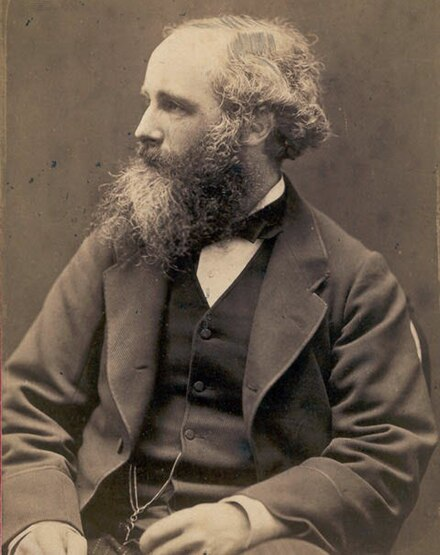
\includegraphics[scale=0.1]{\pathtopartone/graphics/maxwell}
James Clerk Maxwell, (1831 – 1879) was a Scottish physicist with broad interests who was responsible for the classical theory of electromagnetic radiation. This groundbreaking theory marked the first instance where electricity, magnetism, and light were conceptualized as varying expressions of a unified phenomenon.
}
\begin{figure}[h]
\centering
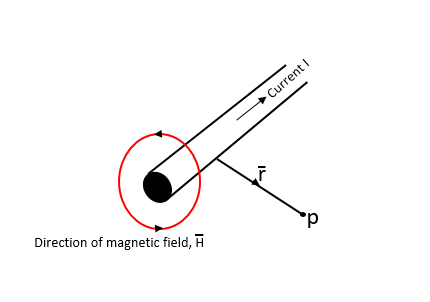
\includegraphics[height=7cm]{\pathtopartone/graphics/currentElement}
\caption{Current carrying element(wire)}
\label{fig:currentelement}
\end{figure}

Now let's consider a current carrying element which is a small piece of wire carrying current(I) with length given by $d\bar{l}$ having direction shown by the arrow in Figure~\ref{fig:currentelement}. At some point in space, P is given by the distance $r$ from the current element.

The magnetic field due to the current element $Id\bar{l}$ is given by the expression
\begin{align}
\boxed{d\bar{H}= \frac{Id\bar{l} \times \hat{\textbf{r}}}{4\pi r^{2}}}\quad (\text{Amp/m})
\label{eqn:magfield}
\end{align} 
This is the \emph{Magneto-motive force (MMF) at that point P}\index{magneto-motive force (mmf)}magneto-motive force (mmf). Analysis From Equation~\eqref{eqn:magfield}
\begin{enumerate}[(i)]
\item The expression shows that the magnetic field is proportional to the current I and the length of the wire through which the current flows but inversely proportional to the square of the distance r from the current element (wire).
\item By applying the right-hand rule, the direction of the magnetic field ($d\bar{H}$) points in the clockwise direction looking in the direction of the current.
\end{enumerate}

The quantity related to the medium parameters is the magnetic flux density ($\bar{B}$) and not the magnetic field ($\bar{H}$). So no matter the medium, $ d\bar{H} $ depends on I, $ d\bar{l} $ and r which are not the medium parameters. 

\section{Magnetic Flux Density $\bar{B}$}\index{magenetic flux density}
This is the product of the permeability of the medium and the magnetic field strength.\\
Mathematically, 
\begin{align}
\boxed{\bar{B} = \mu\bar{H}}\quad\text{(Wb/$m^{2}$) or (Tesla)}
\label{eqn:magflux}
\end{align}
\begin{dmath*}
Where, \newline
\mu = \mu_r\mu_0\newline
\text{$\mu$: Magnetic permeability of the material} \newline
\text{$\mu_r$: Relative permeability of the material} \newline
\text{$\mu_0$: Permeability of free space, $4\pi\times10^{-7}$ H/m}
\end{dmath*}

This relationship allows you to relate the magnetic properties of a material to those of free space. In a vacuum, \( \mu_r \) is equal to 1, and \( \mu \) is equal to \( \mu_0 \). For materials with \( \mu_r \) greater than 1, the material enhances the magnetic field, and for materials with \( \mu_r \) less than 1, the material reduces the magnetic field.

Depending upon the magnetic properties of the material, the value of \index{permeability}permeability changes. So the magnetic flux at point, P, is related to the permeability of the medium and the magnetic field strength. The unit of magnetic flux density is in Tesla or $Weber/m^{2}$.
From Equation~\eqref{eqn:magflux}, we can deduce the following:
\begin{enumerate}[(i)]
\item The magnetic flux density $\bar{B}$ tells us the density of magnetic lines of forces at that particular location. This means it is essentially showing you some kind of vectors that are oriented and hence the reason it is a \index{vector quantity}vector quantity.
\item As we define the electric field as the \emph{force per unit charge due to presence of charges}, we can also define the magnetic field as the \emph{force experienced by a unit magnetic pole placed in the vicinity of the current}, making $\bar{B}$ and $\bar{H}$ vector quantities.
\item In the case of the magnetic field, if the medium is \footnote[2]{An isotropic medium is a medium that has uniform permeability in all directions of the medium }\emph{Isotropic}, $\bar{B}$ and $\bar{H}$ will be in the same direction. Whereas if it is an \footnote[3]{Anisotropic medium is one such that the \index{permeability}permeability and permittivity of the medium are not uniform }\index{\emph{Anisotropic} medium}\emph{Anisotropic} medium $\bar{B}$ and $\bar{H}$ will not be in the same direction. The next one we are looking at is Ohm's law.
\end{enumerate}

\section{Ohm's Law} 
We know that 
\footnote[4]{
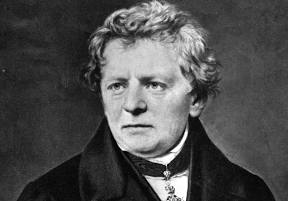
\includegraphics[scale=0.2]{\pathtopartone/graphics/ohms} 
George Ohm, (1789 - 1854), German physicist who discovered the ohms law, named after him. He became a professor of mathematics at the Jesuits’ College at Cologne in 1817.
}

So if we take a medium where the conductivity of the medium is not constant, then it is not meaningful to define the total current for the medium. Normally what we do is, define a quantity called the conduction current density $ \bar{J} $ (i.e. \emph{current flowing per unit area in this conductor}). It has direction which is the direction the current is flowing. 

This current is flowing due to an electric field because it has some electric potential. We have seen that the \index{electric field}electric field is related to the gradient of potential difference.

So if we go from circuital \index{Ohm's law}Ohm's law, we'll have a relationship between voltage and current which have a proportional relationship and also a proportionality constant called \index{\emph{Resistance}}\emph{Resistance}(R).

Now let's establish a relationship between the \index{conduction current density}conduction current density $ \bar{J} $ and \index{electric field}electric field $ \bar{E} $. \\
Mathematically, 
\begin{align*}
I\quad\alpha\quad V \quad\Rightarrow I = \frac{V}{R}
\end{align*} 
Making the `R' subject of the formula, we have that; 
\begin{align}
R = \frac{V}{I} 
\end{align}
\begin{center}
Where R = The introduced constant of proportionality called the \textit{resistance}.
\end{center}
For a conductor of length $\ell$ and the cross-sectional area `A' The resistance is directly proportional to the length and inversely proportional to the cross-sectional area of the conductor.

Mathematically, 
\begin{align*}
R \alpha \frac{\ell}{A}\quad R = \frac{\rho\ell}{A}
\end{align*}
Substitute equation 5.3 into the above formula. We have that;
\begin{align*}
\frac{V}{I} = \frac{\rho\ell}{A}
\end{align*}
Rearranging the equation we have that; 
\begin{align}
\frac{V}{\ell} = \frac{I\rho}{A}
\end{align}
Recall that $\vec{E} = \frac{V}{\L}$ into 5.4, we have that;
\begin{align*}
\vec{E} = \frac{I\rho}{A}
\end{align*}
But the ratio of current to the area is given by a quantity called conduction current density J (i.e $ \frac{I}{A} $ ), Hence
\begin{align*}
\vec{E} = \vec{J}\rho \quad \Rightarrow \vec{J}=\frac{1}{\rho}\vec{E}
\end{align*}

Where the conductivity $ \sigma $ is the the inverse of resistivity and verse versa $ \rho $ (i.e $ \frac{1}{\rho} $ ), 


Hence, $ \sigma = \frac{1}{\rho}$

\boxed{\vec{J} = \sigma \vec{E}}\quad (A/m^{2})\\


This is the \textbf{Conduction current density - The general form of Ohm's law}\index{conduction current density}. Mathematically, it is the product of electric field intensity $\vec{E}$ and $\sigma$ from a reference point where $\sigma$ is the conductivity of the medium(proportionality constant).

In the case of an isotropic medium, both \( \mu_r \) and \( \sigma \) are scalar quantities. This implies that their values remain the same, regardless of the direction.

On the other hand, for an anisotropic medium, where properties vary with direction, \( \mu_r \) becomes a \( 3 \times 3 \) matrix, and \( \sigma \) also transforms into a \( 3 \times 3 \) matrix.

This situation parallels the behavior observed in the electric field, where in an isotropic medium, the displacement vector and electric field align in the same direction. In contrast, for an anisotropic medium, the direction of the electric field may not coincide with that of the displacement vector.

Similarly, in the realm of the magnetic field, if the medium is isotropic, the magnetic flux density (\( \bar{B} \)) and conduction current density (\( \bar{H} \)) align in the same direction. Conversely, in an anisotropic medium, the direction of electric field (\( \bar{E} \)) and the conduction current density (\( \bar{J} \)) are not the same.




\section{The Physical Laws To Maxwell's Equation}
Now from this basic introduction of the parameters, we are set to establish the physical laws mathematically, which when compiled gives Maxwell's equation and these physical laws are the experimental verification of the postulates. There are two ways to get Maxwell's equation
\begin{enumerate}[(i)]
\item You treat it as a mathematical postulate.
\item Try to represent these mathematical laws in appropriate mathematical form to give us Maxwell's equation.
\end{enumerate}

Both ways have merits, that is, if we say Maxwell's equations are mathematical postulates, then they are very exact. However one could ask a question, \emph{How do you get these postulates?} One cannot simply come up with these mathematical formulae, without having a background. So the background is in the physical laws. First, the physical laws came from curiosity towards the relationship between electrical and magnetic fields. So if we go by the picture that Maxwell's equations were guided by the experimented laws, then the advantage is that we always try to see the phenomenon in physical terms. So if we have any electromagnetic phenomenon, and accept that the origin lies in the physical laws, it will always be useful to look at every phenomenon of electromagnetics physically.

However, if you treat these equations more like mathematical postulates then one may get lost in the mathematical manipulation of these equations. So from the exactness point of view, the mathematical postulates have merit, but seeing what is happening physically, first understanding the physical laws and then getting Maxwell's equations.

What we will be doing in this chapter is that would state first the physical laws and then use the vector identities and theorems such as divergence and Stokes theorems, we would try to get the mathematical form and then finally we get Maxwell's equations.

\section{Gauss Law}
This law states that the total displacement(electric flux) coming out of a closed surface is equal to the net charge enclosed by the closed surface.

\begin{figure}[h]
\centering
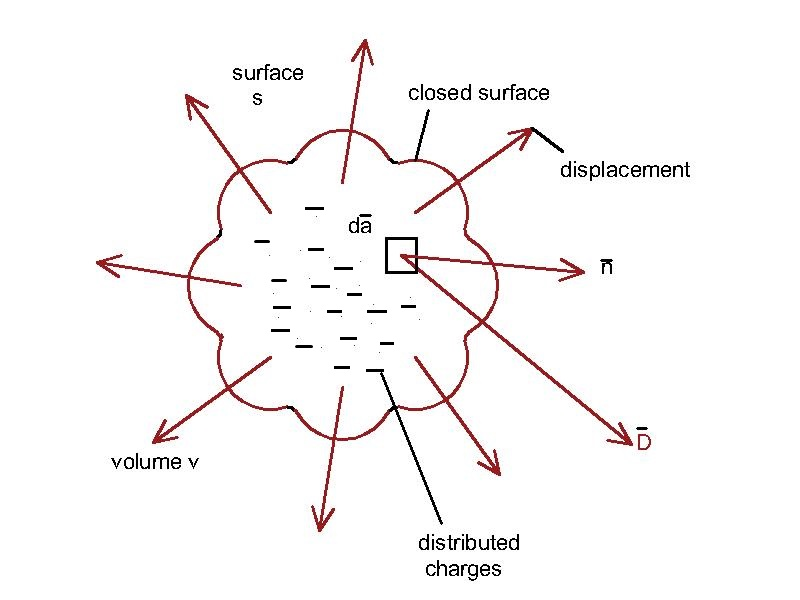
\includegraphics[height=6cm]{\pathtopartone/graphics/g}
\caption{A closed surface showing the direction of displacement vector}
\label{fig:g}
\end{figure}
Total displacement shown by each arrow = net charge enclosed by surface

Mathematically, 
\begin{align}
\Phi_E = Q_{\text{enclosed}}
\end{align}
\begin{align}
\boxed{\oiint_s\bar{D}\cdot{d\bar{a}} = \iiint_v\rho dv}
\end{align}
This is \textbf{Gauss law in integral form}\index{gauss law}.Where $\oiint_s\bar{D}\cdot d\bar{a}$ is the total outward displacement from the total surface. This means using Gauss' law
\footnote[5]{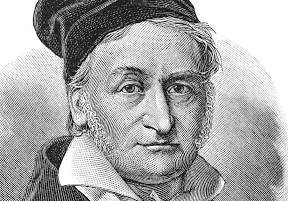
\includegraphics[scale=0.2]{\pathtopartone/graphics/gauss} 
Johann Carl Friedrich Gauss, (1777 – 1855), German mathematician, geodesist, and physicist who made significant contributions to many fields in mathematics and science. Gauss ranks among history's most influential mathematicians. He has been referred to as the "Prince of Mathematicians". 
}

In general, the displacement vector will be varying as a function of the location on the surface, also it will be oriented in different directions. However, the net displacement which is coming out of the surface will be a component of each arrow normal to the surface at that location.

Hence considering a small incremental area ($ d\bar{a} $) on the surface as shown in figure 5.3. ($ d\bar{a} $) has a direction defined by a unit normal $ \hat{n} $ with the direction of the displacement vector given by $ \bar{D} $. The outward displacement coming out from the area is the dot product of $ \bar{D} $ and $ d\bar{a} $. If that is gotten, add all the contributions from others around the surface, and then we have the total displacement coming out of the close surface. Let us say in general, we have charges which are distributed inside this surface and are characterized by a charge density. This is denoted by volume charge density, $ \rho $ (which is representing the density of charges inside the volume). Its S.I. unit of measurement is in coulomb per cubic metres, ($ C/m^{3} $).

In other words, if we add up all the charges inside the volume, we get the charge enclosed by this surface. So integrating the displacement vector over the surface, we get the total outward displacement from this surface. 
Applying\footnote[6]{
$	\iint_A A\cdot d\bar{a} = \iiint (\nabla\cdot \bar{A})dv $. This is the divergence law that was formulated by Gauss.
} divergence theorem to $\iint_s\bar{D}\cdot d\bar{a}$ (Meaning converting surface integral to line volume integral), we will have 
\begin{equation*}
\oiint_s\bar{D} \cdot d\bar{a} = \iiint_v(\nabla\cdot \bar{D})dv
\end{equation*}


Subtitute into equ 5.6
\begin{equation*}
\iiint_v(\nabla\cdot \bar{D})dv = \iiint_v\rho dv
\end{equation*}
\begin{equation*}
\iiint_v(\nabla\cdot \bar{D})dv = \iiint_v\rho dv
\end{equation*}
Collect like terms and factorize out
\begin{equation*}
\iiint_v(\nabla\cdot \bar{D})dv - \iiint_v\rho dv = 0
\end{equation*}
\begin{equation*}
\iiint_v(\nabla\cdot \bar{D})dv - \iiint_v\rho dv = 0
\end{equation*}
\begin{equation*}
\iiint_v(\nabla\cdot \bar{D} - \rho)dv = 0
\end{equation*}
This relationship in the integral can only be
true for all arbitrary volume if and only if $\nabla\cdot\bar{D} - \rho = 0$
\begin{align*}
\nabla \cdot \bar{D} - \rho = 0
\end{align*}
\begin{align}
\boxed{\nabla \cdot \bar{D} = \rho}
\end{align}
Where $\bar{D}$ is the displacement vector\index{displacement vector} and $\rho$ is the volume charge density.\\
From Equation 5.6 and 5.7 we can deduce the following:
\begin{enumerate}[(i)]
\item From the Gauss law in differential form, we saw that the divergence of the displacement vector at any point is related to the charge density at that point. This relationship is called a point relation.
\item The differential form of Gauss law has a limitation as it assumes that, we have a \footnote[7]{ Continuous medium refers to a material or substance that exhibits uniform properties throughout its volume.}continuous media, meaning it will not hold for a \footnote[8]{Discontinuous medium refers to a material or substance that exhibits variations in its properties.}discontinuous media (i.e. the derivative at that point does not exist).
\item While the integral form of Gauss law is applicable in all situations.
\end{enumerate}
\textbf{In conclusion, if the medium is continuous, we apply the differential form. But if not, we apply integral form.}

Considering the relationship between the displacement vector and the electric field, we have 
\begin{align}
\boxed{\bar{D} = \epsilon\bar{E}}
\end{align}
Substituting equation 5.8 into 5.7, we have
\begin{align*}
\nabla \cdot (\epsilon\bar{E}) = \rho
\end{align*}
If we assume that the medium is homogeneous (i.e. $\epsilon$ is not a function of space). Then
\begin{align} 
\boxed{\nabla \cdot \bar{E} = \frac{\rho}{\epsilon}}
\end{align} 
\emph{Gauss law for electric charges for homogeneous medium}\\

Now if we apply Gauss law to magnetic fields and the magnetic charges, we can say that the net magnetic flux coming out of a closed surface is equal to the net magnetic charge enclosed by that surface.\\


However we Know that there are no isolated magnetic poles or charges(\textbf{north and south polesmust and always exist together}).No matter what volume we take, we will always have equal number of north and south poles.\\
So for a closed surface the net magnetic charge is always zero. If we apply Gauss law for the magnetic charges or poles, then there is no net charge enclosed by the closed surface. i.e

\begin{align*}
Q_{\text{enclosed}} = \iiint_v\rho dv = 0
\end{align*}

Hence the net flux coming out of a closed surface for a magnetic field is always equal to zero, because there are no net magnetic charges enclosed by the surface.
\begin{align*}
\phi = \iint_s\bar{B}\cdot d\bar{a} = 0
\end{align*}
Applying divergence theorem to $\iint_s\bar{B}\cdot d\bar{a}$ we have
\begin{align*}
\iiint_v(\nabla \cdot \bar{B})dv = 0
\end{align*}	
For this to be true for any arbitrary volume $(\nabla \cdot \bar{B})$ must be equal to zero.
\begin{align}
\boxed{\nabla \cdot \bar{B} = 0}
\end{align}
\begin{center}
\emph{Gauss law for magnetic charges (magneto-statics)}
\end{center}



\section{Amperes Law}
\footnote[9]{
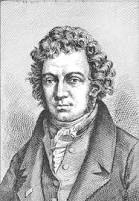
\includegraphics[scale=0.2]{\pathtopartone/graphics/ampere} 
André-Marie Ampère (1775 - 1836) French physicist who founded and named the science of electrodynamics, now known as electromagnetism. He is also the inventor of numerous applications, such as the solenoid and the electrical telegraph.
}

Amperes law is also called \emph{Amperes circuit law} and it states that the magnetomotive force(mmf) around a closed loop is equal to the total current enclosed by the loop.\\
Mathematically, \\
Magnetomotive Force (mmf) = $\oint_c \bar{H} \cdot d\bar{l}$ \\
\begin{figure}[h]
\centering
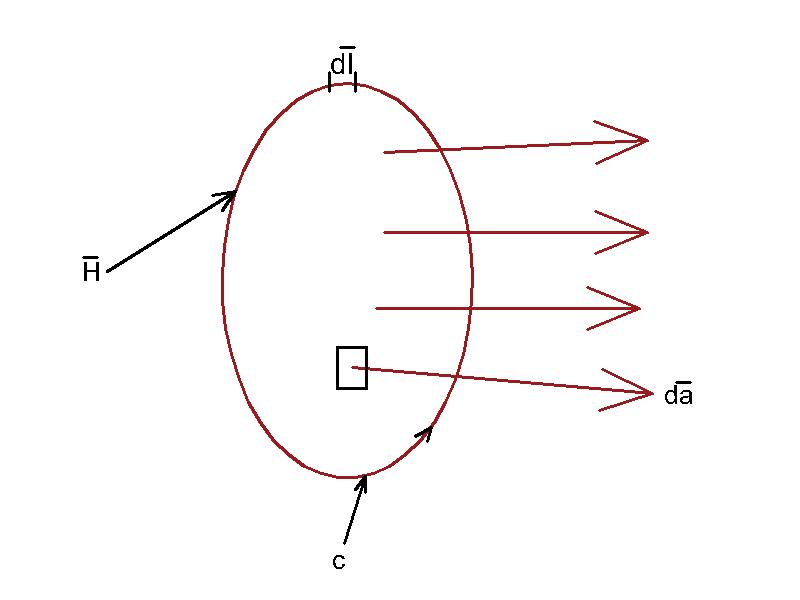
\includegraphics[height=5cm]{\pathtopartone/graphics/j}
\caption{A loop of arbitrary size of non-uniform current}
\label{fig:j}
\end{figure}

Considering a closed loop shown in Figure~\ref{fig:j}, we can calculate the mmf since it is the line integral of the magnetic field along the path created by the closed loop. i.e
\begin{align*}
\Sigma I_{enclosed} &= \oint_c\bar{H}\cdot d\bar{l} = mmf
\end{align*}
Let the total current enclosed by the loop be I.\\
Therefore $\Sigma I_{enclosed} = I$
\begin{equation*}
\Rightarrow I = \oint_c\bar{H}\cdot d\bar{l}
\end{equation*}
Due to these changes, the varying current can be written as current density. The integration of this current density $\bar{J}$ over an enclosed area created by the closed path c? gives us the total current enclosed by contour c.\\
Mathematically,
\begin{equation*}
I = \iint_A\bar{J} \cdot d\bar{a}
\end{equation*}
\begin{equation}
\boxed{\oint_c\bar{H} \cdot d\bar{l} = \iint\bar{J} \cdot d\bar{a}}
\end{equation}
This is Amperes Law in \emph{Integral Form}. Now to get the differential form of Amperes law, we will apply \emph{stroke's theorem} (i.e. converting from line integral to surface integral).
\begin{equation*}
\iint_A(\nabla \times \bar{H}) \cdot d\bar{a} = \iint_A\bar{J} \cdot d\bar{a}
\end{equation*}
\begin{equation*}
\iint_A(\nabla \times \bar{H}) \cdot d\bar{a} - \iint_A\bar{J} \cdot d\bar{a} = 0
\end{equation*}
\begin{equation*}
\iint_A(\nabla \times \bar{H} - \bar{J})d\bar{a} = 0
\end{equation*} 
For this to be true for all arbitrary area, $\nabla \times \bar{H} - \bar{J}$ must be equal to zero
\begin{equation*}
\Rightarrow \nabla \times \bar{H} - \bar{J} = 0
\end{equation*}
\begin{equation}
\boxed{\nabla \times \bar{H} = \bar{J}}
\end{equation}
This is Amperes Law in \emph{Differential Form}\index{amperes law}. Analysis From Equation 5.12
\begin{enumerate}[(i)]
\item What this means is, the curl of $\bar{H}$ is equal to the total conduction current density at that point. Again the differential form of Amperes law is only valid for a continuous medium(meaning if we go to a point and the magnetic field at that point is known(\emph{Point Relationship}), then we can apply the differential form of Amperes law).
\item The integral form of Amperes law is applicable to the finite area enclosed by path c.
\item The above Amperes law in differential form does not show the complete equation for Maxwell's fourth equation. Hence, it will be looked further into in the next chapter.
\end{enumerate}

\section{Faraday's Law of Electromagnetic Induction} 
\footnote{
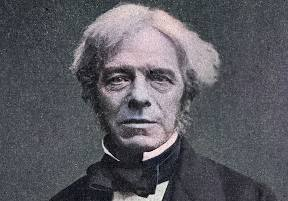
\includegraphics[scale=0.2]{\pathtopartone/graphics/faraday} 
Micheael Faraday, (1791 - 1867), English physicist and chemist whose many experiments contributed greatly to the understanding of electromagnetism.
}

This law states that the total Emf around a closed loop is equal to the rate of change of magnetic flux enclosed by that loop, and that, the direction of emf is such that, the magnetic field produced by this current due to this emf opposes the original magnetic field.
In other words, EMF is the electromotive force induced in the circuit (measured in volts, V). the rate of change of magnetic flux through the coil with respect to time (measured in Weber per second or volt).
$\text{EMF} = -\frac{d\Phi_B}{dt}
$\begin{figure}[h]
\centering
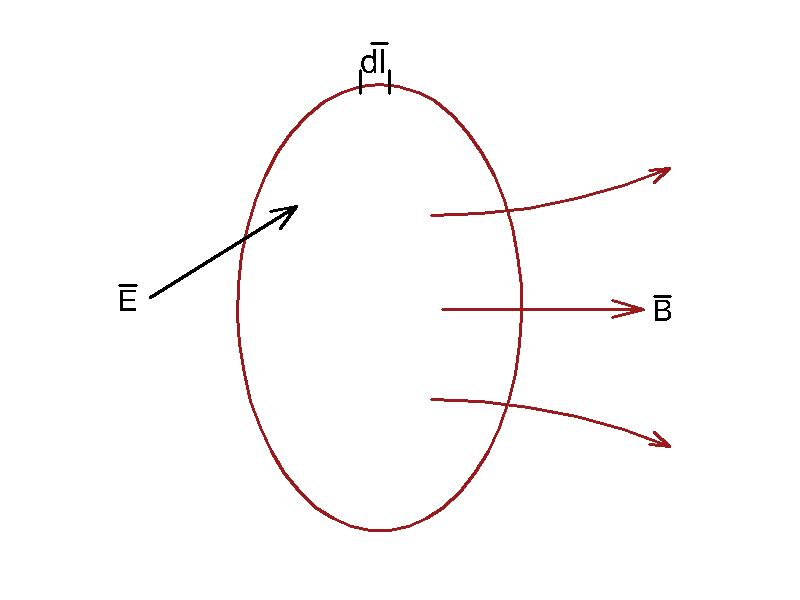
\includegraphics[height=5cm]{\pathtopartone/graphics/k}
\caption{A closed loop used for calculating $\bar{B}$}
\label{fig:k}
\end{figure}

Considering the figure 5.4, the total flux is found by integrating $\bar{B}$ over the area enclosed by that loop. Hence, the rate of change of this flux density is equal to the total emf produced around the loop.

Mathematically,
\begin{dmath}
\text{EMF} = \oint_c\bar{E} \cdot d\bar{l} = -\frac{\delta}{\delta t}(\phi)
\end{dmath}
Where $\phi$ = Total flux enclosed by the loop.
\begin{align}
\boxed{\oint_c\bar{E} \cdot d\bar{l} = -\frac{\delta}{\delta t}(\phi)}
\end{align}
This is the EMF produced by\emph{ $d\bar{l}$}\index{emf}. Analysis From Equation 5.13
\begin{enumerate}[(i)]
\item The negative sign shows that the emf produced is such that, the magnetic field produced by this emf will oppose the original magnetic field. 
\item The magnetic flux can be gotten by integrating the flux density over the area created by the loop to give us the total flux($\phi$) 
\end{enumerate}
mathematically,
\begin{align}
\phi = \iint_A\bar{B} \cdot d\bar{a}
\end{align}
Where $d\bar{a}$ = Incremental Area and $\bar{B}$ = Magnetic flux density.

Substituting equation 5.15 into 5.14 
\begin{align*}
\boxed{Emf = \oint_c\bar{E}\cdot d\bar{l} = -\frac{\delta}{\delta t} (\iint_A\bar{B}\cdot d\bar{a})}
\end{align*}
\emph{This is a general relationship relating to the rate of change of flux}	
\begin{align}
\boxed{\oint_c\bar{E}\cdot d\bar{l} = -\frac{\delta}{\delta t} (\iint_A\bar{B}\cdot d\bar{a})}
\end{align} 
Now let's analyze the general relationship relating to the rate of change of flux.

The rate of change of flux can either happen in two ways.
\begin{enumerate}[(i)]
\item By varying the area of the loop with time while keeping the magnetic flux density $\bar{B}$ constant. This is called the \emph{generator action} (this is how the generator works, where the magnetic flux density is kept constant and by rotating the loop in a magnetic field, the area of the loop changes and we get induced emf).
\item By changing the magnetic flux density $\bar{B}$ with time while the area of the loop remains constant. This is called \emph{transformation action} (This is what happens in a transformer where the size of the coils are not varying as the function of time, but the magnetic flux density induced in this coil varies with time which makes us have induced emf)
\end{enumerate}
Now from the integral form of Faraday's law, let's get its differential form. Hence, we are interested in the time-varying fields (i.e. $\bar{E}$ and $\bar{B}$ fields) and not space-varying fields (loop area) which makes the area not a function of time.
\begin{align*}
{\oint_c\bar{E}\cdot d\bar{l} = -\frac{\delta}{\delta t}(\iint_A\bar{B}\cdot d\bar{a})}
\end{align*}	
Applying \footnote[10]{$\oint_c\bar{A}\cdot d\bar{l} = \iint_s(\nabla \times \bar{A})\cdot d\bar{a}$. This is original form of stokes law.}Stokes Theorem to $\oint_c\bar{E}\cdot d\bar{l}$, we have;
\begin{align*}
\oint_c\bar{E}\cdot d\bar{l} = \iint_A(\nabla\times\bar{E})\cdot d\bar{a}
\end{align*}
\begin{align*}
\iint_A(\nabla\times\bar{E})\cdot d\bar{a} = -\iint_A\frac{\delta \bar{B}}{\delta t}\cdot d\bar{a}
\end{align*}
\begin{align*}
\iint_A(\nabla\times\bar{E})\cdot d\bar{a} = -\iint_A\frac{\delta \bar{B}}{\delta t}\cdot d\bar{a}
\end{align*}
\begin{align*}
\iint_A(\nabla\times\bar{E})\cdot d\bar{a} + \iint_A\frac{\delta \bar{B}}{\delta t}\cdot d\bar{a} = 0
\end{align*}
\begin{align*}
\iint_A\{(\nabla \times \bar{E})+ \frac{\delta \bar{B}}{\delta t}\} d\bar{a} = 0
\end{align*} 
For any arbitrary area $(\nabla \times \bar{E})+ \frac{\delta \bar{B}}{\delta t}$ must be zero for the relationship to be valid.

Hence;
\begin{align*}
\nabla \times \bar{E}+ \frac{\delta \bar{B}}{\delta t} = 0
\end{align*}
\begin{align}
\nabla \times \bar{E} = -\frac{\delta \bar{B}}{\delta t}
\end{align}
This is \emph{Faraday's Law in Differential Form}\index{faraday's law}. For a time-varying medium, if the electric field at a particular point is known, we can find the rate of the magnetic flux density at the location by finding the curl of $\bar{E}$ at that location.

For a non-time varying medium (medium whose permeability $\mu$ does not vary with time), the curl of $\bar{E}$ can give the rate of change of magnetic field strength at that location.\\

What that means mathematically is that,\\


Recall that $\nabla \times \bar{E} = - \frac{\delta\bar{B}}{\delta t}$\\


We know that $\bar{B} = \mu \bar{H}$ $\quad$\\

Substituting $\bar{B}$ into the differential form of Faraday's law, we have	


\begin{align*}
\nabla \times \bar{E} = - \frac{\delta}{\delta t} (\mu\bar{H})
\end{align*}

\begin{align}
\nabla \times \bar{E} = -\mu\frac{\delta \bar{H}}{\delta t}
\end{align}
\emph{This is the Differential form of Faraday's Law of Electromagnetic Induction for a non-time varying medium}

Maxwell's equations describe how electric and magnetic fields interact and propagate through space.He formulated these equations in the 19th century as a set of 20 differential equations. 
\footnote{
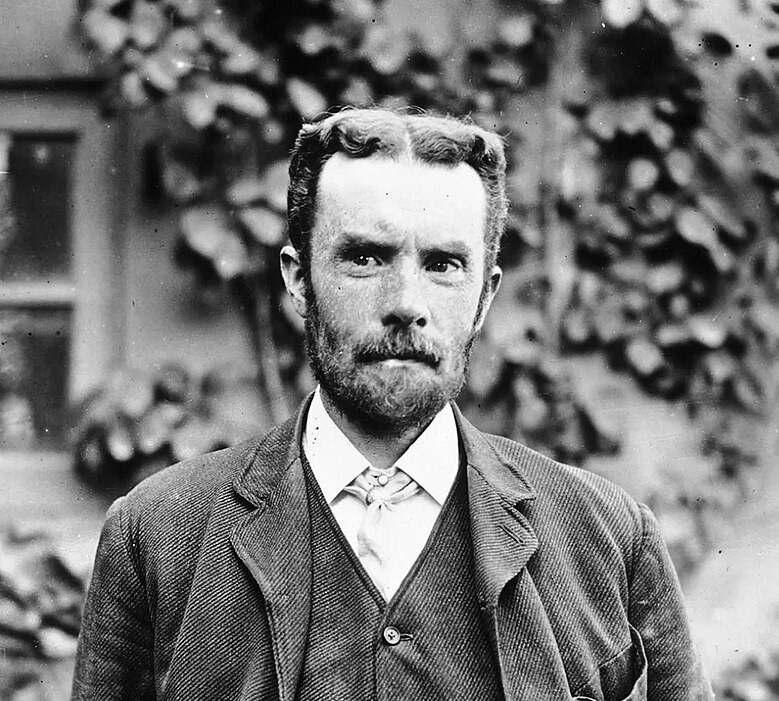
\includegraphics[scale=0.1]{\pathtopartone/graphics/oliver} 
Oliver Heaviside (1850 - 1925), British mathematician and physicist, who invented a new technique for solving differential equations, independently developed vector calculus, and rewrote Maxwell's equations in the form commonly used today.
}


\begin{mdframed}[backgroundcolor=lightblue, linewidth=1pt, hidealllines=true]
\section{Summary}
\begin{enumerate}[(i)]
\item Note that the integral form of all the physical laws discussed in this chapter is applicable in all situations.

\item The origin of the electric and magnetic field is the charge. The effect of the charge is measured by a quantity called the \textbf{\emph{electric field}}.

\item Electric field can be defined as the \emph{force per unit charge due to presence of charges} 

\item When the same charge is kept in motion, it constitutes a current and the pressure of the current is felt by a quantity called \textbf{\emph{magnetic field}}.

\item Magnetic field can also be defined as the \emph{force experienced by a unit magnetic pole placed in the vicinity of the current}.

\item The magnetic field due to the current element $Id\bar{l}$ is given by:
$\boxed{d\bar{H}= \frac{Id\bar{l} \times \hat{\textbf{r}}}{4\pi r^{2}}}\quad (Amp/m)$ 

\item Magnetic field is proportional to the current I and the length of the wire through which the current flows, but inversely proportional to the square of the distance from the current carrying element (wire).

\item Magnetic Flux Density $\bar{B}$ is the product of the permeability of the medium and the magnetic field strength. And is given by the formula;
$$\quad\boxed{\bar{B} = \mu\bar{H}}\quad (Wb/m^{2})$$

\item The general form of Ohms law which is the relationship between conduction current density $\bar{J}$ and electric field Which is given by; $\boxed{\bar{J} = \sigma\bar{E}}\quad (A/m^{2})$

\item The two ways in getting Maxwell's equation
\begin{enumerate}[(i)]
\item	You treat it as a mathematical postulate
\item	Try to represent these mathematical laws in appropriate mathematical form to give us Maxwell's equation.
\end{enumerate}

\item Gauss law states that \emph{the total displacement coming out of a close surface is equal to the net charge enclosed by the closed surface}

\item \begin{align*}
\iint_s\bar{D}\cdot{d\bar{a}} = \iiint_v\rho dv
\end{align*}
\emph{Gauss law in integral form}

\item \begin{align*} 
\nabla \cdot \bar{E} = \frac{\rho}{\epsilon}
\end{align*} 
\emph{Gauss law for electric charges for homogeneous medium}

\item \begin{align*}
\nabla \cdot \bar{B} = 0
\end{align*}
\emph{Gauss law for magnetic charges}

\item Amperes law also called \emph{Amperes circuit law} states that the magneto-motive force(mmf) around a closed loop is equal to the total current enclosed by the loop.

\item \begin{equation*}
\oint_c\bar{H} \cdot d\bar{l} = \iint\bar{J} \cdot d\bar{a}
\end{equation*}
\emph{Amperes Law in Integral Form}

\item \begin{equation*}
\boxed{\nabla \times \bar{H} = \bar{J}}
\end{equation*}
\emph{Amperes Law in Differential Form}

\item Faraday's Law of Electromagnetic Induction states that the total Emf around a closed loop is equal to the rate of change of magnetic flux enclosed by that loop, and that, the direction of emf is such that, the magnetic field produced by this current due to this emf opposes the original magnetic field. 

\item \begin{align*}
\oint_c\bar{E} \cdot d\bar{l} = -\frac{\delta}{\delta t}(\phi)
\end{align*}
\emph{EMF produced by $d\bar{l}$}

\item The negative sign shows that the emf produced is such that, the magnetic field produced by this emf will oppose the original magnetic field. 

\item 
\begin{align*}
\nabla \times \bar{E} = -\frac{\delta \bar{B}}{\delta t}
\end{align*}
\emph{Faraday's Law in Differential Form}
\end{enumerate}
In this chapter, we have seen the four basic laws (Gauss law of Electric charges, the Gauss Law of Magnetic charges, The Amperes Circuit Law and the Faraday Law of Electromagnetic induction) and how we were able to write each of them mathematically and in their integral and differential form using reactor algebra and theorem (Stokes's and Divergent Theorem).
\end{mdframed}


\begin{mdframed}[backgroundcolor=lightblue, linewidth=1pt, hidealllines=true]
\section{EXERCISE}

\begin{ExerciseList}
\Exercise[label={ex1}] A non-uniform charge distribution within a sphere is given by $\rho(r) = \rho_0 \left(1 - \frac{r}{R}\right)$, where $r$ is the radial distance from the sphere's center ($0 \leq r \leq R$) and $\rho_0$ is a constant charge density. Calculate the electric field at a distance $r$ from the center of the sphere.
\hfill\textbf{[$[E = \frac{\rho_0}{3\varepsilon_0}\left(R - \frac{r^2}{R}\right)$]}



%\textbf{Solution:}
%
%Express the differential charge \(dQ\) as a function of the charge density:
%\[
%dQ = \rho(r) \, dV = \rho_0 \left(1 - \frac{r}{R}\right) \cdot 4\pi r^2 \, dr
%\]
%
%Apply Coulomb's law to a differential charge element at a point:
%\[
%dE = \frac{1}{4\pi\varepsilon_0} \frac{dQ}{r^2} = \frac{\rho_0 \left(1 - \frac{r}{R}\right)}{4\varepsilon_0} \cdot \frac{4\pi r^2}{r^2} \, dr
%\]
%
%Integrate the contributions of all differential charges to find the total electric field at the specified point:
%\[
%E = \int_{0}^{R} \frac{\rho_0 \left(1 - \frac{r}{R}\right)}{4\varepsilon_0} \, dr
%\]
%
%
%The electric field $E$ is given by:
\Answer[ref={ex1}]
\[E = \frac{\rho_0}{3\varepsilon_0}\left(R - \frac{r^2}{R}\right)\]

\Exercise[label={ex2}] A long straight wire with a current of $5 \, \text{A}$ is surrounded by a cylindrical surface of radius $0.02 \, \text{m}$. Determine the magnetic field at a distance $0.05 \, \text{m}$ from the wire.
\Answer[ref={ex1}]
\[B = \frac{\mu_0 \cdot 5}{2\pi \cdot 0.05} \, \text{T}\]

\Exercise[label={ex3}] In free space, where there are no charges or currents ($\rho = 0, J = 0$), express Maxwell's equations in differential form.

%\textbf{Solution:}
%The differential form of Maxwell's equations in free space are:
%1. Gauss's Law for Electricity: $\nabla \cdot \vec{E} = 0$
%2. Gauss's Law for Magnetism: $\nabla \cdot \vec{B} = 0$
%3. Faraday's Law: $\nabla \times \vec{E} = -\frac{\partial \vec{B}}{\partial t}$
%4. Ampère's Law with Maxwell's Addition: $\nabla \times \vec{B} = \mu_0 \varepsilon_0 \frac{\partial \vec{E}}{\partial t}$
%
%\textbf{exercise 6: electric field due to a uniformly charged sphere}

\Exercise[label={ex4}] A uniformly charged sphere with a total charge \(q\) and radius \(r\) generates an electric field (\(e\)) at a point outside the sphere. determine the expression for the electric field (\(e\)) as a function of the radial distance (\(r\)) from the center of the sphere.

\Exercise[label={ex6}] Show the relationship that relates the current density with electric field
\Exercise[label={ex7}] Show with diagram the magnetic field due to current element 
\Exercise[label={ex8}] State the laws used to derive Maxwell's equations.
\Exercise[label={ex9}] Show that $\nabla \times \bar{E} = -\frac{\delta \bar{B}}{\delta t}$
\Exercise[label={ex10}] Show that the general form of Ohm's law is 

$\bar{J} = \sigma\bar{E}\quad (A/m^{2})$


\end{ExerciseList}
\end{mdframed}
